\chapter{Introduction} \label{sec:intro}
Positioning assets, such as facilities and equipment, within a pre-defined region, such as a plot of land or a building, in a fashion that is tailoured towards a criteria of optimality for a specific problem is one endeavour that has multiple applications in different fields, primarily due to the benefits it provides. Finding the best possible asset positioning can result in improved operations efficiency, better productivity \cite{El-Baz2004}, and even decreases in expenses \cite{Sahin2011}. As a matter of fact, due to the benefits of asset positioning, \$300 billion dollars have been spent each year on just determining suboptimal locations of buildings and facilities in the United States alone \cite{Asl2015a}. This is further proof of the importance of asset positioning. One entertaining example of said application is showcased by Barriga et al. (2014). In their paper, the authors developed a genetic algorithm that optimized placement of buildings in a StarCraft match. The algorithm produced building placements that allowed the defending player's base to better survive base assaults from the opposing player \cite{Barriga2014}. Developing an open-plan office layout is another application of asset positioning. Chen et al. (2020) also developed a genetic algorithm that generates an open-office layout where the space utilization is maximized as possible \cite{Chen2020}. This task of arranging assets within a given space according to some criteria has a formal term, which is the "facility layout problem", often abbreviated as "FLP". We will be discussing facility layout problems in more detail in this chapter.

FLP is a field that has been researched as early as 1957 (with Koopsman T.C., and Beckman, M. being the first to model the problem) \cite{Kusiak1987}, and there is still active research around it to this day. This research paper is one of the testaments to that. In this research, we will be solving the classical facility layout problem using a recent optimization algorithm called the Grey Wolf Optimization (GWO) algorithm. The specific type of FLP that we will solve is called the unequal area static FLP. The categorization will be discussed later in this paper. The proposed algorithm will then be compared to a genetic algorithm using experimental data used in other related papers.

\section{Facility Layout Problem}
The problem of arranging a set of facilities and/or machines in a pre-determined area, or a set of possible locations (such as in the work of Farmakis, P., and Chassiakos, A. \cite{Farmakis2018}) is called the facility layout problem (FLP). The facilities and/or machines are arranged in such a way that the resulting layout is in line with some criteria or objectives and under certain constraints. These constraints, which must not be violated, include shape, size, orientation, pick-up/drop-off points \cite{Hosseini-Nasab2018}, and usable area \cite{Fernando2015}. Facilities and/or machines must also not overlap. Solutions that satisfy the aforementioned conditions are called feasible solutions \cite{Meller1996}. Figure \ref{flp-illustration} provides an illustration of a facility layout problem. There are other types of facility layout problems, which we will discuss later. The illustration only showcases a continuous type of FLP.

\begin{figure}[h!]
	\centering
	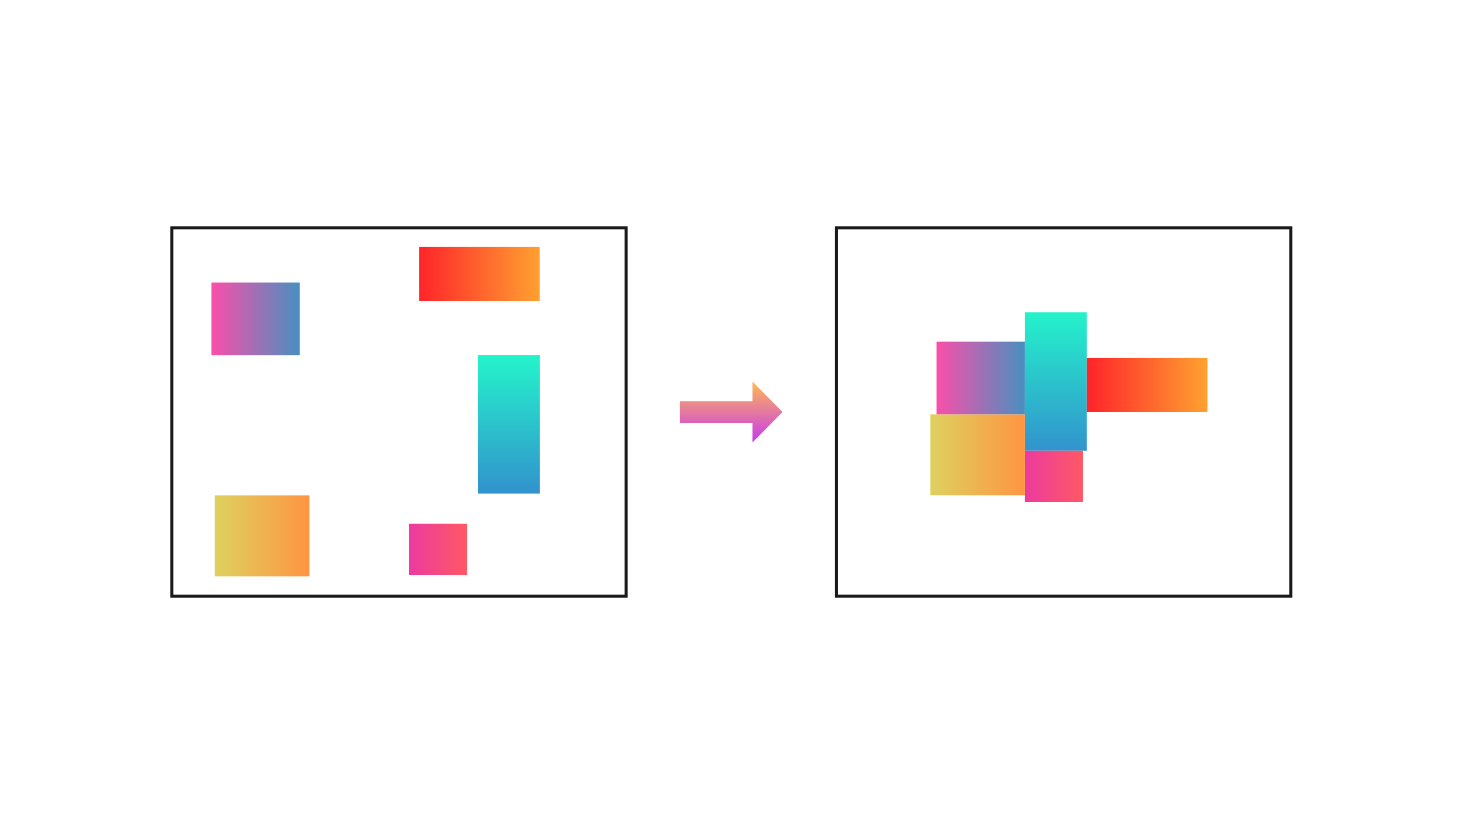
\includegraphics[scale=0.25]{./images/chap01-introduction/flp-illustration.png}
	\caption{An illustration of the facility layout problem (FLP), which seeks to arrange a set of facilities or assets based on some criteria. Note that this illustration only showcases a continuous version of the facility layout problem. There are multiple types of facility layout problems.}
	\label{flp-illustration}
\end{figure}

% TODO: [LOW PRIO] Add a visualization of discrete vs continuous formulations, static vs dynamic, and the other FLP formulations.

Generally, the facility layout problem is considered to be an \textbf{NP-Hard} problem \cite{Drira2007}. Hosseini-Nasab, H., Fereidouni, S., and Fatemi, S. have noted in their systematic review of FLP that most researches dealing with the facility layout problem model their problems either as a quadratic assignment problem (QAP) or a mixed integer programming problem \cite{Hosseini-Nasab2018}. According to Drira, A., Pierreval, H., and Hajri-Gabouj, S., the former is sometimes used in discrete FLP formulations, while the latter is often used in continuous formulations \cite{Drira2007}. Discrete and continuous FLP formulations will be discussed later. \textbf{Quadratic assignment problems} deal with placing $n$ facilities in $n$ locations in such a way that minimizes the assignment cost. The assignment cost is the sum of all facility pairs's flow rate between each other multiplied by their flow rate \cite{QAPDefinition}. This assignment cost is commonly seen in many FLP researches, as we will discuss later. QAP is also known to be an NP-Hard problem \cite{Garey1979}. It should be noted though that \textit{some} instances of QAP are easy to solve \cite{Feizollahi2015}. The other modeling framework, \textbf{mixed integer programming}, can solve problems with both discrete decisions and continuous variables. An example of such problem is the assignment problem \cite{Richards2005}, which the FLP can be classified under. In this formulation, a set of integer and real-valued integers are being optimized based on an objective function that is being minimized or maximized, while satisfying constraints which are linear equations or inequalities \cite{Wolsey2008}. Mixed integer programming, when in the context of optimization, is also known to be NP-Hard \cite{Richards2005}. These two formulations being known to be generally NP-Hard proves that FLP is indeed generally NP-Hard.

The fact that FLP is an NP-Hard problem has resulted in many research works that utilize heuristics (such as simulated annealing and genetic algorithms). Note that there are also works that utilize exact methods, which seek to find the \textit{optimal} solution for a problem. However, the NP-Hard nature of the FLP prevents them from finding the solution in large problems within reasonable time \cite{Asl2015}.

\subsection{The Basic Mathematical Model}
Each problem instances of the facility layout problem naturally will have their own mathematical models tailor-fit for their problem instance. Nevertheless, based on our observations and from readings, most of those models are derivatives of or use (such as in \cite{Garcia-Hernandez2013}, \cite{Lin2019}, and \cite{Navarro2016}) what will be calling a basic minimization function, which is defined as:

$$
\text{min} F = \sum_{i=1}^{n}\sum_{j=1}^{n}c_{ij}f_{ij}d_{ij}
$$

where $N$ is the number of facilities, $c_{ij}$ is the cost of handling materials between locations $i$ and $j$, $f_{ij}$ is the flow rate between $i$ and $j$, and $d_{ij}$ is the distance between the centroids of $i$ and $j$. The distance function may differ from work to work. For example, Liu, J., et. al. uses the Manhattan distance in their work \cite{Liu2018}, while in the work of Ripon, K. S. N., et. al., Euclidean distance was used \cite{Ripon2013}. In works that derive from this formula, such as in \cite{Farmakis2018}, \cite{Solimanpur2008}, and \cite{Peng2018}, it was observed that $d_{ij}$, or a similar variable or expression, is commonly present in the work's objective function while $c_{ij}$ and $f_{ij}$ \textit{may} be present and/or the work uses more or fewer variables.

Drira, A., Pierreval, H., and Hajri-Gabouj, S. note the same observation but showcase a slightly differing formula in their 2007 survey of facility layout problems. Unlike the basic minimization formula above, their formula has $f_{ij}$ and $c_{ij}$ combined. They also note that the function above is typically used in continuous formulations of the FLP. The discrete formulation uses a similar function, but ensures that a facility is only in one location, a location only contains one facility, and makes sure that only pairs of locations that contain facilities contribute to the fitness value of a solution. (The descriptions and the differences of the discrete and continuous formulations are discussed in the next section.) Additionally, they mention that the function is also subject to the following constraints: (1) facilities must obviously not overlap with one another, and (2) the total area used by the facilities must be equal to or less than the allotted area \cite{Drira2007}. These constraints have been observed to be generally in many FLP works.

\subsection{Discrete vs Continuous Formulations}
Solving instances of the facility layout problem requires determining the form of the solution. The form is highly dependent on the problem being solved. Some problems may require a solution that assigns assets to pre-existing locations, while others may require more flexibility. Facility layout problems may be categorized based on the characteristics of these solutions, or formally known as formulations: discrete, and continuous.

In a discrete formulation, the region where the facilities will be laid out are divided into equal rectangular blocks of the same shape and size, or have pre-determined possible facility locations \cite{Drira2007}. Each facility will be given a number of blocks, or be assigned to one facility location, respectively. This formulation, however, does not suit well when the facilities require exact positions and it cannot model facility attributes such as orientation. In problems that have such requirements, a continuous formulation is more appropriate \cite{Hosseini-Nasab2018}. Facilities in a continuous formulation are usually located by either their centroid coordinates, half length, and half width, or by their bottom-left coordinates, length, and width \cite{Drira2007}. This allows for the formulation's flexibility compared to its discrete counterpart. However, this does provide challenges towards ensuring that no two facilities overlap with one another. Discrete formulations do not need to consider this problem due to their inherent characteristics.

\subsection{Static vs Dynamic Facility Layout Problems}
Another categorization for facility layout problems is based on whether the layouts will change over time. There are situations where a regular change of layout over some periods of time is necessitated. The layout of facilities in a construction is one example. As the construction of a building moves to from phase to another, the layout of facilities within the construction site change to better fit the needs of the current phase of construction \cite{Farmakis2018}. A similar need is the motivation behind changing layouts in manufactories. Product demand variations, and even a change in product design can incline a factory's management to reorganize facilities in the building to be more efficient in response to the changes \cite{Pourhassan2017}. There are two categories for the aformentioned criteria. These are: (1) static, and (2) dynamic. We will refer to these categories as \textbf{"period-based layout categories"} in this paper.

The survey of Hoisseini-Nasab et al. (2018) showed that the most common period-based categorization in literature is the static facility layout problem \cite{Hosseini-Nasab2018}. This is likely due to the fact that static facility layout problems are easier to solve than dynamic facility layout problems. Though, it is also possible that many problems just happen to not require consideration of variable changes over time. The \textbf{static facility layout problem}, abbreviated as SFLP, is a type of FLP where variables to be considered such as material handling costs do not change for a considerable amount of time \cite{Perez-Gosende2020}. For this type of problems, only a single layout is generated since no changes are made in the considered variables over time.

However, some industries will find SFLPs inadequate for their needs. There are companies that require adaptability to changes to, for example, product demands. For cases like this, the other category, dynamic facility layout problems are more appropriate \cite{DerakhshanAsl2017}. In the dynamic facility layout problem, abbreviated to DFLP, the variables to be considered change over time, unlike in SFLP. The cost of rearranging facilities are also considered in the problem \cite{Hosseini2016}. The solutions for DFLPs are also divided into time periods, where each period has a different layout. This period may equate to years, seasons, months, or weeks \cite{DerakhshanAsl2017}. DFLPs can also be viewed as extensions of SFLP, since each layout in a period can be viewed as a solution to an SFLP with that period's variables into consideration but with rearrangement costs considered. While most research today is focused on SFLPs, Hosseini-Nasab et al. (2018) recommends that research should deal with DFLPs more these days due to rapid scientific developments, and product changes \cite{Hosseini-Nasab2018}.

\subsection{Other FLP Classifications}
Facility layout problems can also be categorized based on different characteristics. FLPs can be divided by the area of their facilities. The facilities may have the same areas, referred to as equal areas, or have different areas, referred this time to as unequal areas \cite{DerakhshanAsl2017}. They can also be divided based on the possible arrangements of facilities. Some problems may have facilities located only in a single pre-defined row (single-row), or they may be placed anywhere in the region (open field) \cite{Drira2007}. There are multiple classifications for FLP and discussing them in this chapter would take long and dislocate the focus of this paper. Due to that, we would like to refer the reader to the papers of Drira et al. (2007) \cite{Drira2007} and Hosseini-Nasab et al. (2018) \cite{Hosseini-Nasab2018} for more information on FLP classifications.

\section{The Grey Wolf Optimization Algorithm}
In this paper, we will be using the Grey Wolf Optimization algorithm to solve the unequal-area static facility layout problem. As such, we will be introducing the algorithm here for us to gain a better understanding of the algorithm.

\begin{figure}[h!]
	\centering
	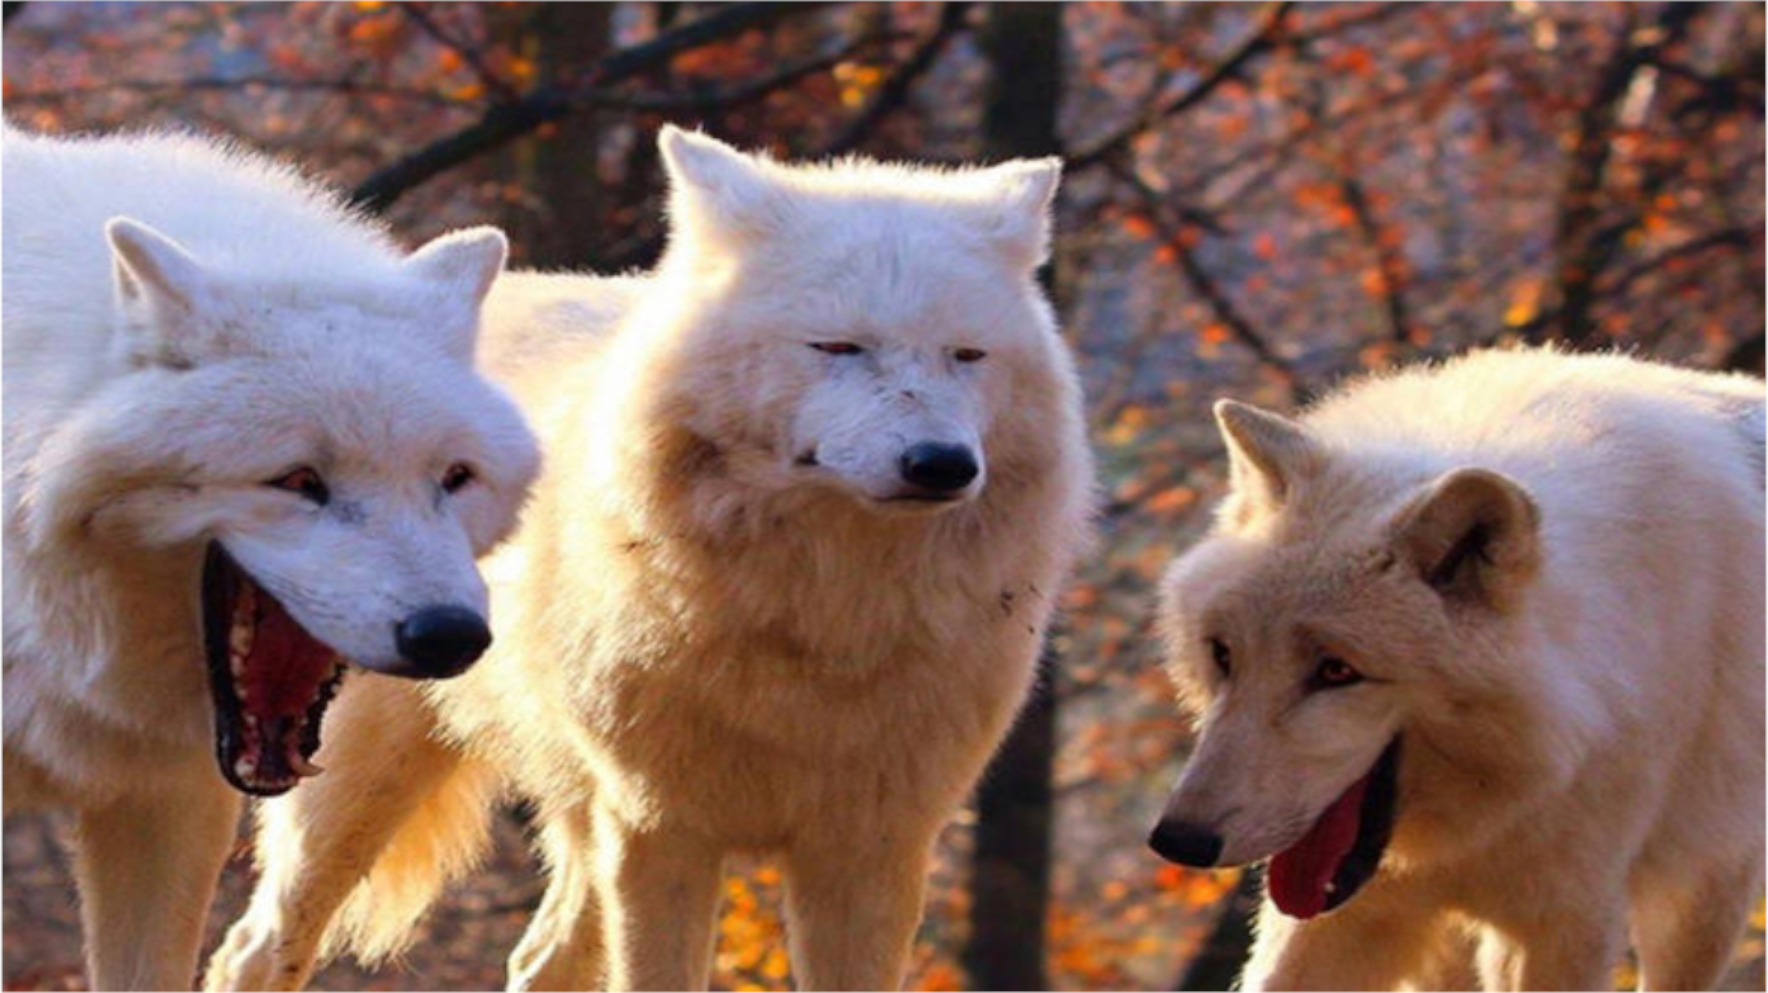
\includegraphics{./images/chap01-introduction/wolves.jpg}
	\caption{The Grey Wolf Optimization algorithm was inspired from the behaviour of grey wolves. Pictured are white wolves, different from grey wolves, but why pass up the opportunity to add a meme in a research paper? Profeshonal.}
	\label{wolves-meme}
\end{figure}

The Grey Wolf Optimization algorithm, abbreviated as GWO, was first conceived by Mirjalili  et al. (2014) in 2014. The optimization algorithm is inspired from the hunting and social behaviour of grey wolves. There is a hierarchy in packs of wolves. Each category in the hierarchy have specific responsibilities. There are four categories: alpha ($\alpha$), beta ($\beta$), delta ($\delta$), and omega ($\omega$). Alpha wolves are responsible for making major decisions for the pack. Every wolf must follow the alpha. However, sometimes the alpha follows other wolves. The second in line is the beta, which ensures the discipline of the pack and advises the alpha. They also command other wolves and reinforces the alpha's commands. The lowest in the hierarchy are the omegas. They must follow the orders of the other wolves, and are the last to eat. Despite their low status, they are still crucial in the pack as their absence causes the pack to face internal fighting and problems. If a wolf is not an alpha, beta, nor omega, they are considered to a delta, the third category in the hierarchy. Deltas may act as scouts, sentinels, elders, hunters, or caretakers. They are also at a category higher than the omegas \cite{Mirjalili2014} \cite{Gupta2018}. The algorithm works by letting the wolves gradually move towards a prey/local optimum solution. At the start, the wolves will be scattered and may likely be too far from a prey. The movement of the wolves, which will be guided by the alpha, beta, and delta wolves (which are closest to a prey/local optimum), will eventually allow them to be in an area where the prey/local optimum is located. As an interesting side note, the inspiration for Grey Wolf Optimization initially came from The Grey \cite{Mirjalili2020}, a movie where survivors of a plane crash must survive, but a pack of grey wolves surround them \cite{TheGreyPlotSummary2011}.

\subsection{Mathematical Model}
The mathematical model assumes the existence of a "pack of wolves". The number of wolves in this pack can be determined by the researcher. Each wolf of this a solution to the problem. We will be delving into the model more in this section, discussing about the model of leadership hierarchy, encircling, and hunting behaviour of grey wolves. The prey being hunted in this scenario is the best solution for a given problem \cite{Mirjalili2014}.

\subsubsection{Leadership Hierarchy}
Solutions are assigned to a certain hierarchy in the mathematical model of GWO. The fittest solution is considered the alpha ($\alpha$), while the second and third fittest are considered to be the beta (\beta) and delta ($\delta$) solutions. The rest of the solutions are referred to as the omega solutions. The leading wolves guide the omegas towards the prey throughout the search process \cite{Gupta2018}.

\subsubsection{Encircling the Prey}
\label{intro-section-encircling-the-prey}
Prey encirclement, which is one of the first steps when grey wolves hunt for their prey, can be modeled with the following:

\begin{align*}
	\vec{X}(t + 1) &= \vec{X_{p}}(t)
					  - \vec{A} \cdot \vec{D}                     \\
	\vec{D}        &= \left | \vec{C} \cdot \vec{X_{p}}(t)
					  - \vec{X}(t) \right | \\
	\vec{A}        &= 2 \cdot \vec{a} \cdot \vec{r_{1}}
					  - \vec{a}                \\
	\vec{C}        &= 2 \cdot \vec{r_{2}}
\end{align*}

where $\vec{X}(t)$ and $\vec{X}(t + 1)$ are the positions of the wolf at the iteration $t$ and $t + 1$ respectively, $\vec{X_{p}}(t)$ represents the location of the prey at the iteration $t$, $\vec{D}$ is the difference vector, $\vec{A}$ and $\vec{C}$ are coefficient vectors, and $\vec{r_{1}}$ and $\vec{r_{2}}$ are uniformly random vectors with the range $\left[ 0, 1 \right]$. $\vec{a}$ is vector that linearly decreases from $2$ to $0$ over the course of iterations \cite{Mirjalili2014}. The original paper on GWO does not specify but Gupta, S. and Deep, K. provided the following equation to specify the decrease of $\vec{a}$ from $2$ to $0$ \cite{Gupta2018}:

$$
\vec{a} = 2 - 2 \cdot \left( \frac{t}{\text{maximum number of iterations}} \right)
$$

Note that the multiplication of vectors in the equations above is a component-wise multiplication, and not a dot product \cite{Mirjalili2020-MathModel}.

\subsubsection{Hunting}
We typically do not know the position of the prey in an abstract search space. As such, it is presumed that the $\alpha$, $\beta$, and $\delta$ solutions have the best idea so far of the position of the prey \cite{Mirjalili2014}. Each wolf updates their positions based on the following equations.

\begin{align}
	\vec{D}_{\alpha} &= \left | \left ( \vec{C}_{1} \cdot \vec{X}_{\alpha} \right ) - \vec{X} \right | \\
	\vec{D}_{\beta} &= \left | \left ( \vec{C}_{2} \cdot \vec{X}_{\beta} \right ) - \vec{X} \right | \\
	\vec{D}_{\delta} &= \left | \left ( \vec{C}_{3} \cdot \vec{X}_{\delta} \right ) - \vec{X} \right | \\
	\vec{X_{1}^{'}} &= \vec{X_{\alpha}}(t) - \vec{A_{\alpha}} \cdot \vec{D_{\alpha}} \\
	\vec{X_{2}^{'}} &= \vec{X_{\beta}}(t) - \vec{A_{\beta}} \cdot \vec{D_{\beta}} \\
	\vec{X_{3}^{'}} &= \vec{X_{\delta}}(t) - \vec{A_{\delta}} \cdot \vec{D_{\delta}} \\
	\vec{X}(t + 1)  &= \frac{\vec{X_{1}^{'}} + \vec{X_{2}^{'}} + \vec{X_{3}^{'}}}{3}
\end{align}

where $\vec{X_{\alpha}}$, $\vec{X_{\beta}}$, and $\vec{X_{\delta}}$ represent the $\alpha$, $\beta$, and $\delta$ solutions \cite{Gupta2018}.

\subsubsection{Exploration and Exploitation}
The exploration phase of metaheuristics is modeled by the search phase, while exploitation is modeled by the attack phase. When $\left| \vec{A} \right| < 1$, or $\vec{C} < 1$, GWO is undergoing exploitation of the search space. Exploitation can be viewed as the wolves approaching towards the prey. On the other hand, when $\left| \vec{A} \right| > 1$, or $\vec{C} > 1$, the algorithm is in the search phase, where the wolves can be viewed as searching for the prey. In the search process, as the number of iterations $t$ reach the maximun possible number, the algorithm tends to focus more on exploitation than exploration. $\vec{A}$ and $\vec{a}$ eventually approach $0$, leaving $\vec{C}$ the sole vector to eventually influence the search exploration. At this point, the algorithm will intensify towards exploitation.

\subsection{Interpretation of GWO in the Abstract Search Space}
In the perspective of an $n$-dimensional abstract search space, we can view preys as local optima (and the value of each prey can be seen as their nutritional value), and the wolves being positioned in some point in the search space. Assuming that we are dealing with the facility layout problem, we can view areas that have infeasible solutions as having higher elevations than those areas with feasible solutions (Note that since it is difficult to visualize and imagine higher-dimensional objects, we are using terms from a three-dimensional plane.). The problem can then be viewed as finding the lowest valley in the search space. Movement of the wolf would be seen in the search space as the traversal of the aforementioned terrain (though the wolves will not struggle in doing so no matter how, from our perspective, difficult the terrain features are to traverse). Wolves in a position where the area is in a high enough elevation would be considered to be having an infeasible solution. When viewed in the FLP space, buildings here may be intersecting with other buildings, among other infeasibility factors. Conversely, those wolves positioned in a low enough area would be considered to have feasible solutions. Buildings in this type of area are not necessarily arranged in a compact manner, but they, at the least, do not violate feasibility criteria. Additionally, given how the GWO is modelled, wolves would not be bothered nor punished when moving towards high elevation/infeasible areas despite coming from a lower/feasible area. This does allow the algorithm to move towards a local optimum faster. To aid understanding of how GWO behaves in the abstract search space, Figure \ref{gwo-in-abstract-search-space-visualization} provides a visualization.

\begin{figure}[h!]
	\centering
	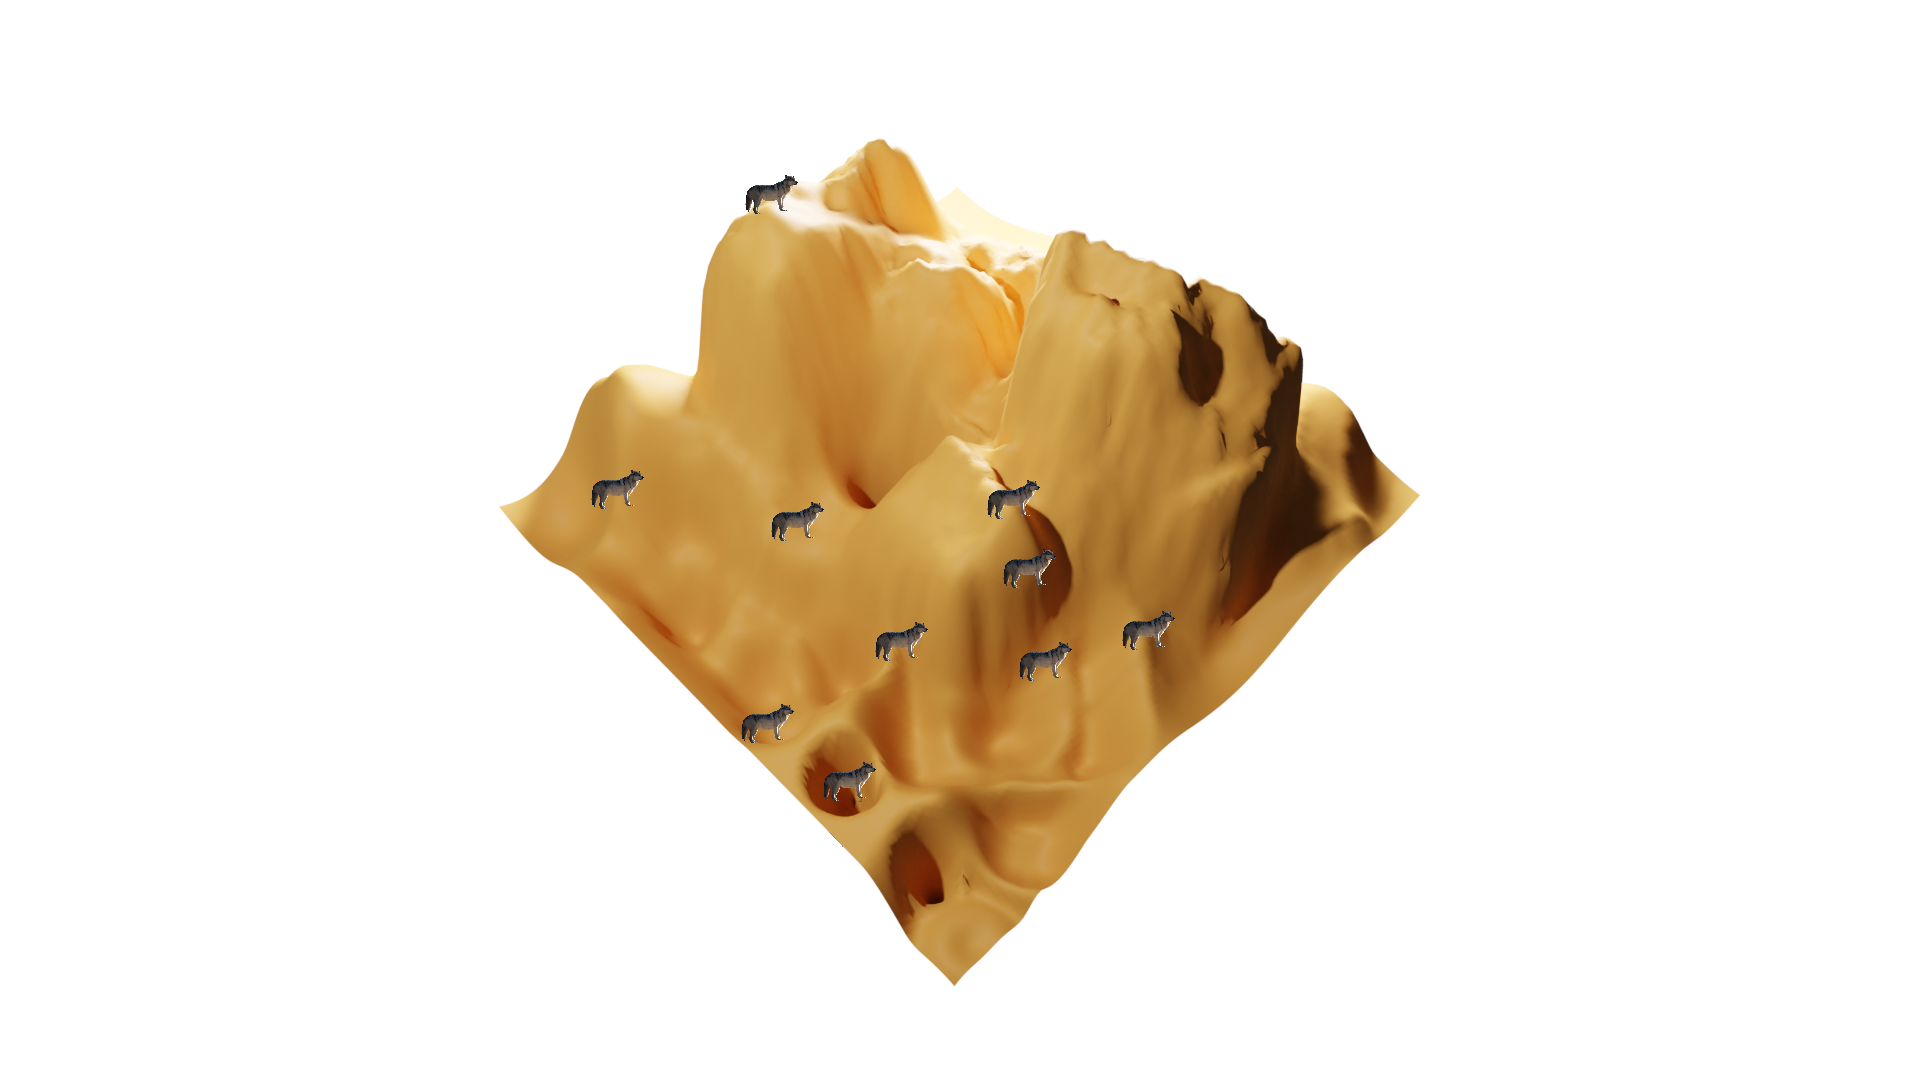
\includegraphics{./images/chap01-introduction/visualization-of-gwo-in-search-space.png}
	\caption{A visualization of how GWO behaves in an $n$-dimensional search space. Throughout the course of the execution of GWO, the wolves will be traversing the terrain (without much difficult, most probably unlike the first author of this manuscript). The topmost wolf has the worst solution, while the bottommost one has the best.}
	\label{gwo-in-abstract-search-space-visualization}
\end{figure}
